\section{Nyutonning ikkinchi qonuni}

\begin{enumerate}

\item Jismning boshqa jism bilan o‘zaro ta’sirlashishi natijasida olgan tezlanishi unga ta’sir qilayotgan kuchga to‘g‘ri proporsional va uning massasiga teskari proporsional. Bu ... .
\begin{enumerate}[label=\Alph*)]
\item Nyutonning III qonuni
\item Impuls saqlanish qonuni
\item Nyutonning I qonuni
\item Nyutonning II qonuni
\end{enumerate}

\item Javoblarda berilgan birliklarning qaysi biri $m/s^2$ birligining o‘rniga ishlatilishi mumkin?
\begin{enumerate}[label=\Alph*)]
\item $kg \cdot m/s$
\item $kg/m$
\item $N/kg$
\item $kg \cdot m/s^2$

\end{enumerate}

\item Quyidagi fikrlarning qaysilari Galileyning nisbiylik prinsipini ifodalaydi:
1) Inersial sanoq sistemalarining tinch yoki to‘g‘ri chiziqli tekis harakatda ekanligini sistemaning ichida o‘tkazilgan har qanday mexanik tajribalar yordamida aniqlab bo‘lmaydi.
2) Barcha inersial sanoq sistemalarida harakat qonunlari bir xil.
3) Noinersial sanoq sistemasining ichida turib uning tinch yoki harakatda ekanligini aniqlab bo‘lmaydi.
4) Barcha noinersial sanoq sistemalarida harakat qonunlari bir xil.
\begin{enumerate}[label=\Alph*)]
\item 2 va 3
\item 1 va 2
\item 2 va 4
\item 1 va 3

\end{enumerate}

\item Tinch turgan jismga bir xil masofada 2 marta katta tezlik berish uchun kuchni necha marta oshirish lozim?
\begin{enumerate}[label=\Alph*)]
\item 2
\item $\sqrt{2}$
\item 3
\item 4
\end{enumerate}

\item Massasi 500 t bo‘lgan passajir poyezdi tormozlanishda tekis sekinlanuvchan harakat qilib, tezligini 60 s da 39,6 km/soat dan 27 km/soat gacha kamaytirgan. Tormozlanish kuchini toping (kN).
\begin{enumerate}[label=\Alph*)]
\item 32,4
\item 56,4
\item 14,2
\item 29,2
\end{enumerate}

\item Massasi 12 kg bo‘lgan tinch turgan jismga 8 s davomida 6 N kuch ta’sir qilgan bo‘lsa, jismning olgan tezlanishi $m/s^2$, shu vaqtda erishgan tezligi ($m/s$), o‘tgan yo‘lini toping (m).
\begin{enumerate}[label=\Alph*)]
\item 0,5; 2; 4
\item 4; 0,5; 2
\item 0,5; 4; 16
\item 25; 4; 2
\end{enumerate}

\item 72 km/soat tezlik bilan to‘g‘ri chiziq bo‘ylab harakatlanayotgan massasi 200 t bo‘lgan poyezdni tormozlash natijasida 10 sekunddan keyin uning tezligi 54 km/soat bo‘lib qoldi. Tormozlash kuchini toping (N).
\begin{enumerate}[label=\Alph*)]
\item $10^3$
\item $10^5$
\item $10^4$
\item $10^8$
\end{enumerate}

\item Massasi 180 kg bo‘lgan arava harakatining birinchi sekundida 15 sm yo‘l bosdi. Tezlanish beruvchi kuchni toping (N).
\begin{enumerate}[label=\Alph*)]
\item 12
\item 48
\item 27
\item 54
\end{enumerate}

\item 20 N kuch jismni tezligini 5 s ichida 1 m/s dan 2 m/s gacha oshirib bergan bo‘lsa, jismning massasi (kg) qanchaga teng?
\begin{enumerate}[label=\Alph*)]
\item 100
\item 20
\item 50
\item 200
\end{enumerate}

\item Avtomobil 1 $m/s^2$ tezlanish bilan harakat qilmoqda. Massasi 70 kg bo‘lgan odam o‘rindiq suyangichga qanday kuch (N) bilan bosadi?
\begin{enumerate}[label=\Alph*)]
\item 140
\item 35
\item 70
\item 700
\end{enumerate}

\item Massasi 1500 t bo‘lgan poyezd 57,6 km/soat tezlik bilan harakat qilmoqda va tormozlanish paytida 200 m yo‘lni o‘tib to‘xtaydi. Poyezd ikki marta kam yo‘lni o‘tib to‘xtashi uchun tormozlanish kuchi qanday o‘zgarishi kerak?
\begin{enumerate}[label=\Alph*)]
\item $6,2 \cdot 10^5$ N; ikki baravar ortishi kerak
\item $3,3 \cdot 10^4$ N; ikki baravar ortishi kerak
\item $9,6 \cdot 10^5$ N; ikki baravar kamayishi kerak
\item $9,6 \cdot 10^5$ N; ikki baravar ortishi kerak
\end{enumerate}

\item Massasi 1 kg bo‘lgan jismning harakat tenglamasi $x = 2t + 15t^2$ (m) ko‘rinishga ega. Jismga ta’sir etuvchi kuchni aniqlang (N).
\begin{enumerate}[label=\Alph*)]
\item 2
\item 7,5
\item 15
\item 30
\end{enumerate}

\item Yengil avtomobilning massasi 2 t, yuk avtomobilniki 8 t. Yuk avtomobilining tortish kuchi yengil avtomobilnikiga qaraganda 2 marta katta bo‘lsa, avtomobillarning tezlanishlarini taqqoslang.
\begin{enumerate}[label=\Alph*)]
\item yengil avtomobilning tezlanishi 2 marta katta
\item yengil avtomobilning tezlanishi 4 marta katta
\item yengil avtomobilning tezlanishi 2 marta kichik
\item yengil avtomobilning tezlanishi 4 marta kichik
\end{enumerate}

\item Massasi 2 t bo‘lgan traktor bo‘sh prisepga 0,6 $m/s^2$ tezlanish, 2,5 t yukli xuddi shunday prisepga esa 0,3 $m/s^2$ tezlanish beradi. Bo‘sh prisepning massasini aniqlang (kg).
\begin{enumerate}[label=\Alph*)]
\item 300
\item 500
\item 900
\item 1200
\end{enumerate}

\item Massasi 4 t bo‘lgan bo‘sh yuk avtomobili 0,3 $m/s^2$ tezlanish bilan harakatlana boshladi. Agar avtomobil o‘sha tortish kuchida joyidan 0,2 $m/s^2$ tezlanish bilan qo‘zg‘alsa, avtomobilga ortilgan yukning massasi qanday (t)?
\begin{enumerate}[label=\Alph*)]
\item 1
\item 4
\item 5
\item 2
\end{enumerate}

\item Vertikal yo‘nalishda pastga 250 m balandlikdan 20 m/sek tezlik bilan otilgan jism 20 sm chuqurlikda yerga kiradi. Agar jism massasi 2 kg bo‘lsa, tuproqning o‘rtacha qarshilik kuchini aniqlang (N).
\begin{enumerate}[label=\Alph*)]
\item 14200
\item 1800
\item 47500
\item 27000
\end{enumerate}

\item Massasi 2 kg bo‘lgan jism tezligining o‘zgarish grafigiga asosan, harakatning har bir bosqichida jismga ta’sir etayotgan kuchning proyeksiyasi $F(x)$ ni toping (N).
\begin{enumerate}[label=\Alph*)]
\item 1; 0; -2
\item 4; 0; -2
\item 5; 0; -2
\item 2; 0; -4
\end{enumerate}

\item Inersial sanoq sistemasida jismga ikki kuch ta’sir etmoqda. Quyidagi vektorlardan qaysi biri jism tezlanishi yo‘nalishini to‘g‘ri tasvirlaydi?

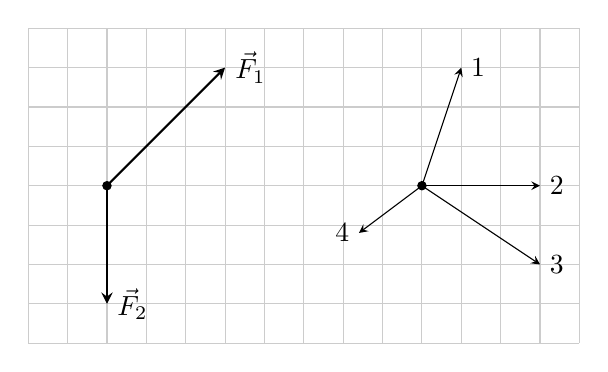
\begin{tikzpicture}[>=stealth, scale=1]

\draw[step=0.5, gray!40, thin] (-1,-2) grid (6,2);
    % --- Chap tomondagi kuchlar sistemasi ---
    \begin{scope}[xshift=0cm]
        \filldraw (0,0) circle (1.5pt); % Jism
        
        % F1 kuchi (yuqoriga va o'ngga)
        \draw[->, thick] (0,0) -- (1.5, 1.5) node[right] {$\vec{F}_1$};
        
        % F2 kuchi (pastga)
        \draw[->, thick] (0,0) -- (0, -1.5) node[right] {$\vec{F}_2$};
    \end{scope}

    % --- O'ng tomondagi yo'nalishlar (variantlar) ---
    \begin{scope}[xshift=4cm]
        \filldraw (0,0) circle (1.5pt); % Markaziy nuqta
        
        % 1-yo'nalish (yuqoriga va biroz o'ngga)
        \draw[->] (0,0) -- (0.5, 1.5) node[right] {1};
        
        % 2-yo'nalish (o'ngga)
        \draw[->] (0,0) -- (1.5, 0) node[right] {2};
        
        % 3-yo'nalish (pastga va o'ngga - to'g'ri javob)
        \draw[->] (0,0) -- (1.5, -1) node[right] {3};
        
        % 4-yo'nalish (pastga va chapga)
        \draw[->] (0,0) -- (-0.8, -0.6) node[left] {4};
    \end{scope}
\end{tikzpicture}

\begin{enumerate}[label=\Alph*)]
\item 3
\item 4
\item 2
\item 1
\end{enumerate}

\item Avtodrezina ikkita platformani tekis tezlanuvchan harakat bilan olib borayotib tortish kuchi 1,8 kN ga teng bo‘lgan. Platformalarning massalari 12 va 8 t. Bu ikki platforma orasidagi tirkash moslamasi qanday kuch bilan tortiladi (kN)?
\begin{enumerate}[label=\Alph*)]
\item 0,8
\item 0,48
\item 0,32
\item 0,72
\end{enumerate}

\item Rasmda to‘rtta kuch vektori tasvirlangan. Qaysi kuch olib tashlansa qolgan kuchlarning teng ta’sir etuvchisi nolga teng bo‘ladi?


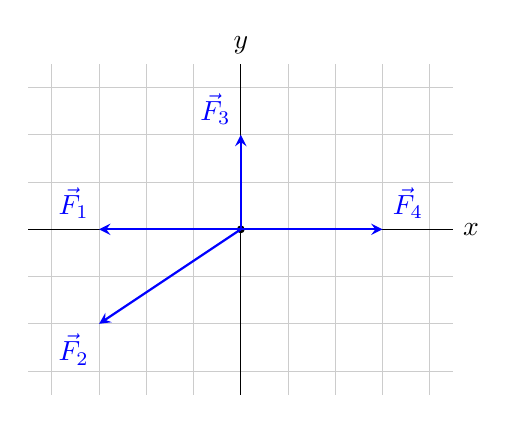
\begin{tikzpicture}[>=stealth, scale=0.6]
    % Orqa fondagi panjara (grid)
    \draw[step=1, gray!40, thin] (-4.5,-3.5) grid (4.5,3.5);
    
    
    \draw (-4.5,0) -- (4.5,0) node[right] {$x$};
    \draw (0,-3.5) -- (0,3.5) node[above] {$y$};

    % Markaziy nuqta
    \filldraw (0,0) circle (2pt);

    % Kuch vektorlari (manbadagi koordinatalar asosida)
    % F1: chapga 2 birlik
    \draw[->,  thick, blue] (0,0) -- (-3,0) node[above left] {$\vec{F}_1$};
    
    % F2: chapga 3 birlik, pastga 2 birlik
    \draw[->,  thick, blue] (0,0) -- (-3,-2) node[below left] {$\vec{F}_2$};
    
    % F3: yuqoriga 2 birlik
    \draw[->,  thick, blue] (0,0) -- (0,2) node[above left] {$\vec{F}_3$};
    
    % F4: o'ngga 3 birlik
    \draw[->, thick, blue] (0,0) -- (3,0) node[above right] {$\vec{F}_4$};

\end{tikzpicture}

\begin{enumerate}[label=\Alph*)]
\item $\vec{F}_1$
\item $\vec{F}_2$
\item $\vec{F}_3$
\item $\vec{F}_4$
\end{enumerate}

\end{enumerate}


\begin{table}[h!]
\centering
\caption{Test savollarining to'g'ri javoblari jadvali}
\begin{tabular}{|l|c|c|c|c|c|c|c|c|c|c|}
\hline
\textbf{Test №} & 1 & 2 & 3 & 4 & 5 & 6 & 7 & 8 & 9 & 10 \\ \hline
\textbf{Javob}  & D & C & A & D & D & C & B & D & A & C \\ \hline
\hline
\textbf{Test №} & 11 & 12 & 13 & 14 & 15 & 16 & 17 & 18 & 19 & 20 \\ \hline
\textbf{Javob}  & D & D & A & B & D & D & B & A & D & A \\ \hline
\end{tabular}
\end{table}













\section{Nyutonning uchinchi qonuni}


\begin{enumerate}

\item Nyutonning 3-qonunining eng to'g'ri yozilgan ta'rifini ko'rsating.
\begin{enumerate}[label=\Alph*)]
\item Ikki jismning o'zaro ta'sir kuchlari bir to'g'ri chiziq bo'ylab qarama-qarshi yo'nalgan.
\item Ikki jismning o'zaro ta'sir kuchlari miqdor jihatidan o'zaro teng.
\item Ikki jismning o'zaro ta'sir kuchlari miqdor jihatidan teng va bir to'g'ri chiziq bo'ylab qarama-qarshi yo'nalgan.
\item Ikki jism bir-biri bilan miqdor jihatidan teng va bir to'g'ri chiziq bo'ylab qarama-qarshi yo'nalgan kuchlar bilan tortishadi.
\end{enumerate}

\item Massasi M bo'lgan jism gorizontal tekislikda tinch turibdi. Bu holatda jism hosil qiladigan bosim kuchi bilan tayanch reaksiya kuchining modul jihatidan tengligi Nyutonning nechanchi qonuni asosida tushuntiriladi?
\begin{enumerate}[label=\Alph*)]
\item I
\item II
\item III
\item I, III
\end{enumerate}

\item Massalari 2 kg va 5 kg bo'lgan jismlar o'zaro ta'sirlashish natijasida birinchi jism $4 m/s^2$ tezlanish olgan bo'lsa, ikkinchi jismning olgan tezlanishini toping ($m/s^2$).
\begin{enumerate}[label=\Alph*)]
\item 10
\item 1,6
\item 4
\item 5
\end{enumerate}

\item Massalari 2 kg va 5 kg bo'lgan jismlar o'zaro ta'sirlashish natijasida ikkinchi jism $4 m/s^2$ tezlanish olgan bo'lsa, birinchi jismning olgan tezlanishini toping ($m/s^2$).
\begin{enumerate}[label=\Alph*)]
\item 10
\item 1,6
\item 4
\item 5
\end{enumerate}

\item Radiuslari bir xil bo'lgan temir ($\rho_t = 7800 kg/m^3$) va mis ($\rho_m = 8900 kg/m^3$) sharlarning o'zaro ta'sirlashuv vaqtida olgan tezlanishlari modullarining nisbati nimaga teng bo'ladi?
\begin{enumerate}[label=\Alph*)]
\item 1,5
\item 89/78
\item 1
\item 25/31
\end{enumerate}

\item Dinamometrning ikki tomoniga qarama-qarshi yo'nalishda 4 N dan kuchlar qo'yilgan. Dinamometr necha nyutonni ko'rsatadi?
\begin{enumerate}[label=\Alph*)]
\item 8
\item 0
\item 4
\item 5
\end{enumerate}

\item Mushtingiz bilan devorni 20 N kuch bilan ursangiz devor sizning mushtingizga qanday kuch bilan ta'sir ko'rsatadi (N)?
\begin{enumerate}[label=\Alph*)]
\item 40
\item 20
\item 10
\item 0
\end{enumerate}

\item Ikki kishi devorga mahkamlangan dinamometrlarni tortib, mos ravishda 700 N va 800 N kuch ko'rsatishlari mumkin. Agar ular dinamometrni shu uchidan bir tomonga qarab tortsa, dinamometr qancha kuchni ko'rsatadi (N).
\begin{enumerate}[label=\Alph*)]
\item 700
\item 800
\item 1500
\item 100
\end{enumerate}

\item Ikki kishi devorga mahkamlangan dinamometrlarni tortib, mos ravishda 700 N va 800 N kuch ko'rsatishlari mumkin. Agar katta kuchni ko'rsatgan kishi dinamometrning bir uchidan ushlab qimirlamay tursa (reaksiya kuchi vazifasini bajarsa), dinamometrni ikkinchi uchidan ikkinchi kishi bor kuchi bilan tortsa, dinamometr necha Nyuton kuchni ko'rsatadi?
\begin{enumerate}[label=\Alph*)]
\item 700
\item 800
\item 1500
\item 100
\end{enumerate}

\item Ikki kishi devorga mahkamlangan dinamometrlarni tortib, mos ravishda 300 N va 600 N kuch ko'rsatishlari mumkin. Agar katta kuchni ko'rsatgan kishi dinamometrning bir uchidan ushlab qimirlamay tursa (reaksiya kuchi vazifasini bajarsa), dinamometrni ikkinchi uchidan ikkinchi kishi bor kuchi bilan tortsa, dinamometr necha Nyuton kuchni ko'rsatadi?
\begin{enumerate}[label=\Alph*)]
\item 300
\item 700
\item 500
\item 100
\end{enumerate}

\item Agar birinchi po'lat sharning radiusi ikkinchi po'lat sharning radiusidan 2 marta katta bo'lsa, ularning markaziy to'qnashish vaqtida tezlanishlari modullarining nisbati nimaga teng bo'ladi?
\begin{enumerate}[label=\Alph*)]
\item 2
\item 3
\item 4
\item 8
\end{enumerate}

\item Ikkita bir xil vaznsiz dinamometrga 10 kg massali yuk osilsa, yuqoridagi va pastgi dinamometrlar necha nyutonni ko'rsatadi?

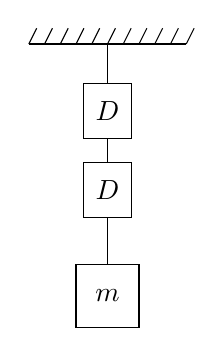
\begin{tikzpicture}
    % Tayanch (ship)
    \draw[thick] (0,4) -- (2,4);
    \foreach \x in {0,0.2,0.4,0.6,0.8,1.0,1.2,1.4,1.6,1.8,2.0}
        \draw (\x,4) -- (\x+0.1,4.2);

    % Birinchi dinamometrgacha bo'lgan ip
    \draw (1,4) -- (1,3.5);

    % Yuqoridagi dinamometr (D)
    \draw (0.7, 2.8) rectangle (1.3, 3.5);
    \node at (1, 3.15) {$D$};

    % Dinamometrlar orasidagi ip
    \draw (1, 2.8) -- (1, 2.5);

    % Pastdagi dinamometr (D)
    \draw (0.7, 1.8) rectangle (1.3, 2.5);
    \node at (1, 2.15) {$D$};

    % Yukka boruvchi ip
    \draw (1, 1.8) -- (1, 1.2);

    % Yuk (m)
    \draw (0.6, 0.4) rectangle (1.4, 1.2);
    \node at (1, 0.8) {$m$};

\end{tikzpicture}

\begin{enumerate}[label=\Alph*)]
\item 100; 50
\item 10; 10
\item 100; 200
\item 100; 100
\end{enumerate}

\item Qayiqdan qirg‘oqqa sakragan odam oldinga harakatlanganda qayiq orqaga siljiydi. Bu hodisa Nyutonning nechanchi qonuni bilan tushuntiriladi?
\begin{enumerate}[label=\Alph*)]
\item Birinchi qonun
\item Ikkinchi qonun
\item Uchinchi qonun
\item Butun olam tortishish qonuni
\end{enumerate}

\item Miltiqdan o‘q otilganda miltiqning orqaga tepishi nimaning natijasidir?
\begin{enumerate}[label=\Alph*)]
\item Inersiyaning
\item Nyutonning ikkinchi qonunining
\item Nyutonning uchinchi qonunining
\item Ishqalanish kuchining

\end{enumerate}

\item Muz ustida turgan ikki bola bir-birini itarsa, ular qarama-qarshi tomonga harakatlana boshlaydi. Bu hodisa qaysi qonun bilan izohlanadi?
\begin{enumerate}[label=\Alph*)]
\item Nyutonning birinchi qonuni
\item Nyutonning uchinchi qonuni
\item Nyutonning ikkinchi qonuni
\item Energiyaning saqlanish qonuni
\end{enumerate}


\end{enumerate}


\begin{table}[h!]
\centering
\begin{tabular}{|l|c|c|c|c|c|c|c|c|c|c|c|c|c|c|c|}
\hline
\textbf{Test №} & 1 & 2 & 3 & 4 & 5 & 6 & 7 & 8 & 9 & 10 & 11 & 12&13&14&15 \\ \hline
\textbf{Javob}  & C & C & B & A & B & C & B & C & A & A & D & D&C&C&B \\ \hline
\end{tabular}
\end{table}